\section{ЗАСОБИ РОЗРОБКИ}


Галузь інформаційних технологій рушила далеко вперед за останні декілька десятків років.
У тому числі в питанні засобів розробки. 


Зараз існує багато інструментів, які покликані
полегшити та покращити досвід написання коду та усі цикли розробки програмного забезпечення
в цілому. З'явилося чимало мов програмування загального призначення,
які все ж зайняли свої певні ніші й використовуються переважно в якійсь одній галузі,
незважаючи на своє загальне призначення. Оскільки ресурси розробників цих мов не необмежені,
вони фокусуються на конкретних функціях та особливостях і реалізовують саме їх. Таким чином,
навіть мови загального призначення відрізняються одна від одної і підходять краще під ті,
чи інші задачі. Тому дуже важливо не бездумно користуватися найпростішим, чи тим інструментом,
який ти знаєш краще, а обирати і вивчати ті, які найкраще підходять під поставлену задачу.

\subsection{Мова програмування Python}
Для написання цієї роботи використовувалася мова програмування Python. Це інтерпретована
об'єктно-орієнтована мова програмування високого рівня зі строгою динамічною типізацією.
Ця мова відома, перш за все, за свою відносну простоту та низький поріг входу,
а також за високий темп розробки, внаслідок свого динамічного та інтерпритованого характеру.
Оскільки ця мова інтерпритується віртуальною машиною, а не компілюється під конкретну
операційну систему, це робить її також \hyperlink{term1}{крос-платформенною}.
Але основна причина чому мова Python чудово підходить для задач обробки природної мови
та статистичного аналізу - це велика спільнота науковців та розробників, які створили чималу
кількість бібліотек та інструментів які підвищують рівень абстракції і дозволяють сфокусуватися
на предметі дослідження і не відволікатися на низькорівневі речі, як-от
\hyperlink{term2}{парсинг} вихідних файлів.
Говорячи про версію, використовувалася версія 3.9, яка є зворотньо не
сумісною з другою, але великою її перевагою є модуль типізації, який
активно використовувався при розробці.

\subsubsection{Пакетний менеджер Pip}
Пакетні менеджери автоматизують рутинну роботу по установці та управлінню
залежностями проекту. Усі пакети зберігаються в централізованому
реєстрі. Це значно спрощує пошук необхідної бібліотеки адже досить провести
пошук по такому реєстру і можна гарантовано знайти десяток бібліотек навіть
на найспецифічнішу тему. Особливо в таких популярних мовах програмування як
Python. Пакетний менеджер Pip не доступний із глобального контексту, після
установки мови Python. На справді, це і не потрібно адже за замувчуванням
він встановлює залежності в папку користувача операційної системи, що може
призводити до небажаного засмічування системи. Набагато продуктивніше
використовувати Pip у комбіннації з віртуальним середовищем мови Python.
При створенні такого середовища, крім того що можна мати версію мови, яка
відрізняється від тієї що встановлена за замовчуванням в операційній системі,
Pip туди встановлюється за замовчуванням. Відповідно і завантажує
всі пакети не у папку користувача, а у це віртуальне середовище.

Для того, щоб автоматизувати процес розгортання проекту, використовується
текстовий файл requirements.txt, в якому вказуються всі установлені пакети
та їх версії. Вказувати версію дуже важливо адже із розвитком встановлених
бібліотек може мінятися і їхній інтерфейс. Відповідно з часом проект може
просто перестати працювати. Для вирішення цієї проблеми використовується
стандарт найменнування версій Semantic versioning, скорочено семвер.
Згідно з цим стандартом, версії поділяються на 3 семантичні
частини ``x.x.x''. Де перша частина означає основну версію, яка змінюється
тільки після глобальних змін, які напряму впливають на кінцевий інтерфейс
програми. Такі зміни ще називають тими, які порошують зворотню сумісність.
Друга частина означає неосновну версію. Її змінюють коли запроваджують
зміни, які не порушють зворотню сумісність, а тільки додають новий функціонал.
Зазвичай цю версію можна зміннювати, не боячись, що проект не запуститься.
Третя частина означає патч версію. Її змінюють коли виправляють несправності
чи небажану поведінку коду. Зазвичай бажано мати найсвіжішу патч версію,
щоб не мати критичних вразливостей у себе в проекті.

\subsubsection{Інтегроване середовище розробки PyCharm}
Як основне середовище розробки використовувався редактор PyCharm, 
розроблений компанією JetBrains. На відміну від багатьох інших
популярних редакторів коду, PyCharm, як то кажуть, поставляється з батарейками
в комплекті. В ньому є все необхідне для комфортної розробки на мові
Python. Окрім стандартного функціоналу, який присутнній у інших
редакторах, наприклад підсвітка синтаксису мови програмування,
PyCharm також має вбудований термінал, що значно спрощує розробку
коннсольних застосунків, таких як ця робота. Але найголовніше,
що у PyCharm встановлений і сконфігурований мовний сервер Pyright,
який аналізує абстрактне синтаксне дерево коду і пропонує підказки,
автодоповнення та автоматично імпортує модулі. Також PyCharm не потрібно
додатково конфігурувати, наприклад, він автоматично визначає віртуальне
середовище мови Python і індексує модулі що в ньому знаходяться,
включно зі станндартною бібліотекою мови Python відповідної версії.

\subsection{Система контролю версій Git}
Система Git без сумніву є одним із найголовніших засобів розробки 21 століття. Проблема
керування версіями виникла ще за часів написання перших програм. І загострилася із
експоненційним ростом складності програмного забезпечення.

Системи контролю версій зберігають історію зміни файлу або набору файлів для того,
щоб у майбутньому була змога
повернутися до певної збереженої версії. Системи контролю версій гарантують можливість
відновити втрачені чи пошкоджені файли і легеко повернути їх у робочий стан. Найпростіше
рішення контролю за версіями - це звичайне копіювання файлів у іншу директорію. Це, мабуть,
є найрозповсюдженішим способом вирішення цієї проблеми, внаслідок своєї простоти.
Але у такого способа є фатальні недоліки. По-перше, дуже просто заплутатися у створених
директоріях. По-друге, файли досі зберігаються на локальному носії, що у разі
несправності призведе до втрати усіх файлів. По-третє, такий підхід зовсім 
не масштабується. Із розростанням кодової бази і складності програмного продукту кількість
файлів та директорій буде на стільки великою, що тільки на копіювання буде витрачатися
величезна кількість часу, не кажучи вже про управління і підтримку такої системи.
Тому очевидно що такий підхід непрактичний і нежиттєздатний для розробки програмного
забезпечення.

На заміну такого підходу прийшли системи контролю версій. Перші з них мали звичайну
базу даних, у якій зберігалася інформація про зміну файлів. Однак вони все ще не
вирішували проблему втрати файлів у разі несправності носія. Розподілені системи
по типу Git покликані вирішити і цю проблему. Основною ідеєю таких систем є те, що
усі дані зберігаються не в одному місці (на локальному носії, чи то на віддаленому
сервері), а копіюються на пристрої кожного розробника, що дає змогу відновити усю історію
змін.

Система Git має багато переваг над конкурентами. Завдяки своєму унікальному підходу
до зберігання інформації про зміни файлів, вона може запропонувати такі функції,
які не доступні багатьом конкурентам внаслідок обмеженості їх архітектури.
На відміну від більшості систем, Git зберігає знімки станів кожного з файлів, а не історію
зміни, рис. \ref{img:git_snapshots}.

\begin{figure}[ht]
  \begin{center}
    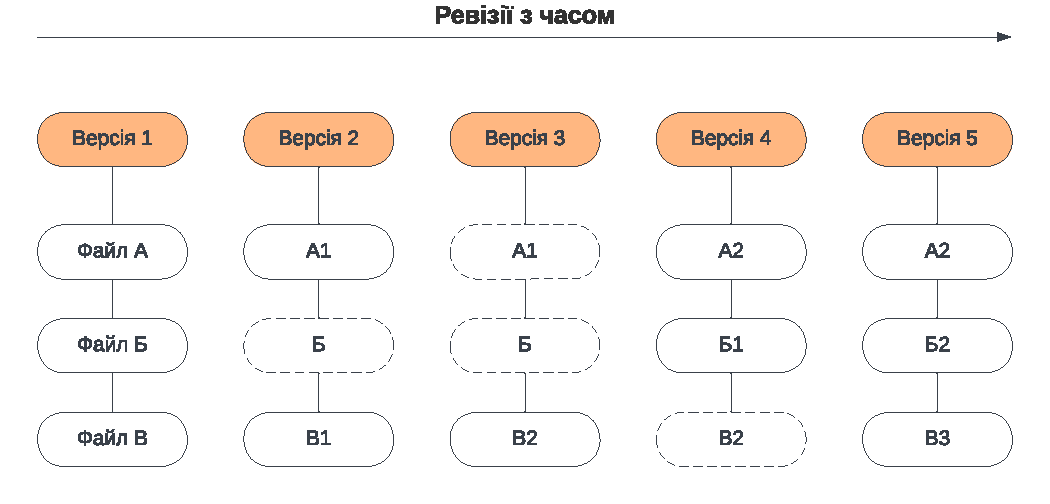
\includegraphics[width=\linewidth]{git-snapshots.pdf}
  \end{center}
  \caption{Зберігання даних у вигляді знімків станів}
  \label{img:git_snapshots}
\end{figure}

На перший погляд це може здатися затратним по об'єму пам'яті, який знадобиться для 
копіювання знімків станів. Але, по-перше,
Git проводить внутрішні оптимізації та не копіює знімки
файлів що не змінилися. Замість цього в репозиторії зберігаються малі за розміром посилання
на попередні знімки файлів. По-друге, хоча це і справді трохи збільшує розмір репозиторію,
на практиці, різниця майже непомітна адже звичайні текстові файли, які часто знаходяться
під контролем такої системи, займають дуже мало місця. По-третє, такі незначні недоліки
повністю нівелюються функціоналом, який подібна система може запропонувати.

Незважаючи на свій розподілений характер, всі операції в системі Git здійснюються локально,
без підключення до мережі, тому інформація з інших ком'ютерів, на яких відслідковується
такий самий репозиторій, не потрібна. Як наслідок, усі операції здійснюються практично
моментально. Що дуже контрастує із іншою системою Subversion, у якій вся інформація
зберігається на віддаленому сервері, і будь-яка зміна потребує оновлення на цьому
віддаленому сервері.

У системі Git для всіх даних, перед збереженням, зберігається так звана контрольна сума.
Це дає змогу забезпечити цілісність даних та високий рівень контролю над тим
вмістом, який потрапляє до репозиторію. Також, Git, як правило, тільки додає
інформацію, тому дуже складно зробити невідворотню дію. Якщо щось потрапило до
репозиторію, то це гарантовано можна буде відновити. Це дає можливість не боятися
за стан локальних файлів та експерементувати. Користувач модифікує файли у робочій папці,
які на цей момент мають статус ``такі, що не відслідковуються'' (unstaged). Система,
як зрозуміло із назви, не відслідковує зміни в таких файлах. Їх дуже просто видалити
і повернутися до стану файлів, які мають статус ``зафіксовані'' (commited).

Основною перевагою системи Git, серед багатьох інших, є система створення гілок, яка
дозволяє вести розробку паралельно і мати декілька версій проекту одночасно. Це унікальна
особливість Git, яка стала можливою завдяки згаданому раніше підходу збереження даних
у вигляді знімків станів (рис. \ref{img:git_snapshots}). Гілки у Git є дуже легковісними
вказівниками на контрольну суму зафіксованих файлів, тому операція створення гілки
відбувається миттєво. Переключання гілок ніяк не впливає на стан файлів репозиторія,
але змінює стан файлів у робочій папці. Потужна система гілок Git виводить розробку
програмного забезпечення на якісно новий рівень та сильно виділяє Git з-поміж аналогів
систем контролю версій.

Список функцій системи Git не обмежується переліченими вище, але у цій роботі 
використовувалися тільки згадані можливості.

\subsubsection{Інтернет хостинг GitHub}
Вихідний код програмного продукту цієї роботи розміщено на платформі GitHub.
Це найбільший хостинг Git репозиторіїв та, одночасно, майданчик для співробітництва
мільйонів розробників зі всього світу.

Оскільки Git є розподіленою системою, так зване ``джерело правди'' знаходиться у кожного,
хто має відповідний репозиторій на своєму комп'ютері. Але дуже зручно мати ``головний''
репозиторій, де синхронізуються всі зміни. І у разі втрати локальних даних, їх дуже просто
відновити.

На сайті GitHub зберігається точна копія локального репозиторія і відрізняєтся лише тим,
що там система Git виступає у якості сервера. На ньому не ведеться безпосередня розробка,
туди потрапляють дані із всіх клонованих репозиторіїв. А GitHub, в свою чергу, надає
можливість управління цим віддаленим репозиторієм через систему запитів на злиття
(pull request) та можливістю створити захищені гілки, в які напряму не можна нічого
зливати. Це можна буде зробити тільки після схвалення оглядачів. Тому будь-хто може
взяти участь у розробці проекту що зацікавив. Але в той самий час є запобіжники у
вигляді вищезгаданих механізмів, які не дозволяють зіпсувати чи якось нашкодити
проекту, шляхом написання неякісного коду, або такого, що не відповідає стандартам
відповідного проекту.

\subsection{Утиліти Universal Dependencies для обробки даних}

Проект Universal Dependencies має багато корисних інструментів, розроблених спільнотою.
Половина з них написана мовою Python, яка також використовувалася для розробки цієї роботи, інша половина написана мовою Perl.
Найкориснішими з них, мабуть, є скрипт валідації та нормалізації
файлів. Адже для багатьох мов, включаючи українську, де символи закодовані
кирилицею, важливо мати правильне кодування файлу, для коректного його
відображенння. У нашому випадку, це кодування UTF-8.

\begin{itemize}
  \item validate.py - Зчитує файл CoNLL-U і перевіряє, чи він відповідає
  специфікації UD. Цей скрипт повинен запускатися з кодом мови, для 
  української - це \texttt{uk}, і повинні існувати відповідні списки із
  специфічними до банку дерев характеристиками і відносини залежностей, щоб 
  перевірити, чи вони дійсні.
  
  \item eval.py - Оцінює точність токенізатора/лемматизатора/теггера/парсера
  UD щодо даних золотого стандарту.
  
  \item check\_sentence\_ids.pl - Зчитує файли CoNLL-U і перевіряє, чи кожне
  речення має унікальний ідентифікатор у коментарі sent\_id.
  Усі файли одного банку дерев (репозиторію) необхідно надати відразу, щоб
  перевірити унікальність ідентифікатора для всього дерева.
  
  \item normalize\_unicode.pl - Перетворює Unicode у нормалізовану форму NFC.
  Можна застосувати до будь-якого текстового файлу, закодованого UTF-8,
  включаючи CoNLL-U. У результаті, якщо є комбінації символів, які за
  визначенням мають виглядати однаково, для представлення гліфа буде
  використовуватися та сама послідовність байтів, що покращує точність моделей
  (якщо вони також застосовуються до нормалізованих даних).
  
  \item conllu-stats.pl - Зчитує файл CoNLL-U, збирає різні статистичні дані
  та виводить їх.
  
  \item mwtoken-stats.pl - Зчитує файл CoNLL-U, збирає статистику багатослівних токенів і виводить їх.
  
  \item enhanced\_collapse\_empty\_nodes.pl - Зчитує файл CoNLL-U, видаляє
  порожні вузли та налаштовує розширені графи так, щоб шлях, який проходить
  один або кілька порожніх вузлів, стискався в одне ребро.
  
  \item overlap.py - Порівнює два файли CoNLL-U та шукає речення, які
  зустрічаються в обох (дослівні копії послідовностей лексем). Деякі банки
  дерев, особливо ті, де оригінальний текст був отриманий з Інтернету, містять
  дублікати. Цей інструмент допомагає з’ясувати, чи потрапив один із дублікатів у тренуваьні дані, а інший — у розробку чи тестування.
  
  \item conllu\_to\_text.pl - Перетворює файл у форматі CoNLL-U на звичайний
  текст, перенесений у рядки по 80 символів 
  (але вихідний рядок буде довшим, якщо є слово, довше за ліміт).
  
\end{itemize}